\documentclass[addpoints]{exam}

\usepackage{amsmath}
\usepackage{amssymb}
\usepackage{geometry}
\usepackage{venndiagram}
\usepackage{graphicx}
\usepackage{tikz}
\usepackage{listings}
\usepackage{xcolor}
\usepackage{tabularx}
\usepackage{multicol}
\usepackage{multirow}
\usepackage{colortbl}
\lstset { %
    language=C++,
    backgroundcolor=\color{black!5}, % set backgroundcolor
    basicstyle=\footnotesize,% basic font setting
}

% Header and footer.
\pagestyle{headandfoot}
\runningheadrule
\runningfootrule
\runningheader{Computer Architecture}{Homework 2}{CE/CS - 321/330}
\runningfooter{}{Page \thepage\ of \numpages}{}
\firstpageheader{}{}{}

% \boxedpoints
\printanswers
\qformat{} %Comment this to number questions, uncomment this to not number questions

\newcommand\union\cup
\newcommand\inter\cap

\title{Computer Architecture}
\author{Ali Muhammad Asad \\ aa07190} 
\date{Homework 2}
\begin{document}
\maketitle

\begin{center}
    \gradetable[h][questions]
\end{center}
\begin{sloppypar}
% \newpage
\begin{questions}
    \question[10]
    \textbf{Q1} [10 marks]\\ You are given the following register values: \\ \hspace*{6mm}x5 = 0x00000000AAAAAAAA, x6 = 0x1234567812345678

    (a) For the register values shown above, what is the value of x7 for the following sequence of \hspace*{6mm}instructions? \\ \hspace*{7mm} \textit{slli}  x7, x5, 4  \\ 
    \hspace*{7mm} \textit{or}  x7, x7, x6 
    
    \vspace*{2mm}
    (b) For the register values shown above, what is the value of x7 for the following sequence of \hspace*{6mm}instructions? \\ 
    \hspace*{7mm} \textit{slli} x7, x6, 4 \\ \hspace*{7mm} \textit{andi} x7, x7, 7

    \vspace*{2mm}
    (c) For the register values shown above, what is the value of x7 for the following sequence of \hspace*{6mm}instructions? \\ \hspace*{7mm} \textit{srli} x7, x5, 3 \\ \hspace*{7mm} \textit{andi} x7, x7, 0x\text{FE}
    \begin{solution}
        The above values translated into binary are: \\ 
            x5 = 0000000000000000000000000000000010101010101010101010101010101010 \\ 
            x6 = 0001001000110100010101100111100000010010001101000101011001111000

        \begin{parts}
            \part  
            \textbf{\textit{slli} x7, x5, 4} $\implies$ shifting logical left the value of x5 by 4 bits: \\ 
            x5 = 0000000000000000000000000000101010101010101010101010101010100000 \newline [x5 = 0x0000000AAAAAAAA0] \\ 
            Storing this in x7,\\ x7 = 0000000000000000000000000000101010101010101010101010101010100000 

            \textbf{\textit{or} x7, x7, x6} $\implies$ perform bitwise or on x7 and x6 and store it in x7: \\ 
            \begin{tabular}{|c|c|}
                \hline 
                x7 & 0000000000000000000000000000101010101010101010101010101010100000 \\ \hline
                x6 & 0001001000110100010101100111100000010010001101000101011001111000 \\ \hline
                \textit{or} & 0001001000110100010101100111101010111010101111101111111011111000 \\ \hline
            \end{tabular}

            The bitiwse \textit{or} value is stored in x7. Therefore,\\ x7 = 0001001000110100010101100111101010111010101111101111111011111000 \\ $\implies$ \boxed{\text{x7 = 0x1234567ABABEFEF8}}

            \part 
            \textbf{\textit{slli} x7, x6, 4} $\implies$ shifting logical left the value of x6 by 4 bits: \\ 
            x6 = 0010001101000101011001111000000100100011010001010110011110000000 \newline [x6 = 0x2345678123456780] \\ Storing this in x7, \\ 
            x7 = 0010001101000101011001111000000100100011010001010110011110000000

            \textbf{\textit{andi} x7, x7, 7} $\implies$ perform AND operation between the value stored in x7, and the immediate value 7, that is 0b111. \\
            \begin{tabular}{|c|c|}
                \hline x7 & 0010001101000101011001111000000100100011010001010110011110000000 \\ \hline 7 & 0000000000000000000000000000000000000000000000000000000000000111 \\ \hline \textit{andi} & 0000000000000000000000000000000000000000000000000000000000000000 \\ \hline
            \end{tabular}

            So, x7 = 0000000000000000000000000000000000000000000000000000000000000000 \\ $\implies$ \boxed{\text{x7 = 0x00000000}}

            \part  
            \textbf{\textit{srli} x7, x5, 3} $\implies$ shift right logical immediate the value in x5 by 3 bits and store it in x7. \\ 
            x5 = 0000000000000000000000000000000000010101010101010101010101010101 \\ $ \implies $ x5 = 0x0000000015555555. 
            Storing this in x7, \\ x7 = 0000000000000000000000000000000000010101010101010101010101010101

            \textbf{\textit{andi} x7, x7, 0xFE} $\implies$ perform AND operation between the value stored in x7, and the immediate value 0xFE $\implies$ 11111110 \\
            \begin{tabular}{|c|c|}
                \hline x7 & 0000000000000000000000000000000000010101010101010101010101010101 \\ \hline 0xFE & 0000000000000000000000000000000000000000000000000000000011111110 \\ \hline \textit{andi} & 0000000000000000000000000000000000000000000000000000000001010100 \\ \hline
            \end{tabular}

            So, x7 = 0000000000000000000000000000000000000000000000000000000001010100 \\ $\implies$ \boxed{\text{x7 = 0x0000000000000054}}
        \end{parts}
    \end{solution}
\newpage
    \question[10]\textbf{Q2} [10 marks] \\ 
    Here is a small code in C code: 

    while (you\underline{\hspace{2mm}}can\underline{\hspace{2mm}}do\underline{\hspace{2mm}}this\underline{\hspace{2mm}}homework[i] $ == $ k) \\ \hspace*{12mm} i $ += 1 $;

    You are given that the array named ``you\underline{\hspace{2mm}}can\underline{\hspace{2mm}}do\underline{\hspace{2mm}}this\underline{\hspace{2mm}}homework'' has some base address stored in x25. i and k correspond to register x22 and x24. Please translate the above C code to an equivalent assembly code with appropriate instructions. Write explanation for your code.
    \begin{solution}

        \underline{Assumptions:} i is in x22 and has the value 0 to it initially, k is in x24, base address of array is in x25, and the array stores doublewords.

        Before storing or performing any operations, we will have to first load the value in ``you\underline{\hspace{2mm}}can\underline{\hspace{2mm}}do\underline{\hspace{2mm}}this\underline{\hspace{2mm}}homework[i]''. Moreover, before indexing, we will constantly have to change the offset on each iteration so that on each iteration of the loop, the next doublword is accessed from the array. Therefore, first we will have to declare \texttt{i} with an offset, and then increment it on each iteration with the value of 8 since one doubleword is of 8 bytes, therefore, the next value from the array will be after an offset of 8 on each iteration. [For our ease, we will refer to ``you\underline{\hspace{2mm}}can\underline{\hspace{2mm}}do\underline{\hspace{2mm}}this\underline{\hspace{2mm}}homework[i]'' as array[i]]

        RISC-V Code: 

        \begin{tabular}{r l l} 
            \texttt{Loop:} & \texttt{slli x10, x22, 3} & \#Temp register x10 = i * 8 \\ 
            & \texttt{add x10, x10, x25} & \# x10 = address of array[i] \\ 
            & ld x11, 0(x10) & \#Temp register x11 = array[i] \\ 
            & \texttt{bne x11, x24, Exit} & \#go to Exit if array[i] $\neq$ k \\ 
            & \texttt{addi x22, x22, 1} & \# i += 1 \\ 
            & \texttt{beq x0, x0, Loop} & \# go to Loop \\ 
            \texttt{Exit:} & & 
        \end{tabular}

        The first line shifts the value of \texttt{i} by 8, as $ 2^3 = 8 $ and one doubleword is of 8 bytes, therefore, the next doubleword will be after an offset of 8. Moreover, it will branch back to this line while array[i] $\neq$ k. \\ The second line gets the address of array[i] and adds the value of \texttt{i} to it to get the next doubleword, or the next value as we need to add the value of \texttt{i} stored in \texttt{x10} with the base of array[i] in \texttt{x25}. \\ 
        The third line loads the value of array[i] into another temporary register \texttt{x11} to perform further operations on it. \\ 
        The fourth line compares the value in \texttt{x11} with the value of k, and if array[i] is not equal to k, then it Exits, otherwise it moves onto the next instruction. \\ 
        The fifth line increments the value of \texttt{i} by 1 for the next iteration. \\ 
        The sixth line branches back to start of the Loop meaning an iteration has been completed. \\ 
        The seventh line contains the Exit label, and if the Exit label has been called, then we will move out of the loop and towards whatever instruction comes next.
    \end{solution}

    \question[10]\textbf{Q3} [10 marks]
    \\ Translate the following C procedure to RISC-V assembly code. 

    Use a minimum number of instructions. Assume that the values of a, b and i are in registers x5, x6, and x7, respectively. Also, assume that register x10 holds the base address of the array D. Preserve the values of temporary registers used in the procedure using stack. 
    
\begin{lstlisting}
long long int(long long int a,long long int b,long long int i,long long int D[]){
    int temp = a + b + i;
    if (a > b)
        D[a] = b;
    else
        D[b] = a;
}
\end{lstlisting}
    \begin{solution}
        
        \underline{Assumptions:} a is in x5, b is in x6, i is in x7, and base address of D is in x10. 

        RISC-V Code:

        \hspace*{1mm} \texttt{li x10, 0x100} \hspace*{5mm} \#Load D's base address \\ 
        \hspace*{1mm} \texttt{jal x1,long\underline{\hspace*{2mm}}long\underline{\hspace*{2mm}}int } \\ 
        \hspace*{1mm} \texttt{j exit}

        \hspace*{1mm} \texttt{long\underline{\hspace*{2mm}}long\underline{\hspace*{2mm}}int:}

        \begin{tabular}{c l l}
            & \texttt{addi sp, sp, -8} & \#Reserving space on stack \\
            & \texttt{sd x11, 0(sp)} & \#temp register x11 onto stack \\
            & \texttt{add x11, x5, x6} & \#Temp register x11 = a + b \\ 
            & \texttt{add x11, x11, x7} & \#Temp register x11 = a + b + i \\ 
            & \texttt{bge x5, x6, IF} & \#if (a $>$ b), move onto IF statement \\ 
            & \# Else statement: &  \\
            & \texttt{slli x6, x6, 3} & \#b = b * 8 for offset as long long int is of 8 bytes \\ 
            & \texttt{add x6, x6, x10} & \#add offset to the base address in x10 \\ 
            & \texttt{sd x6, 0(x5)} & \#D[a] = b \\ 
            & \texttt{beq x0, x0, Exit} & \# Exit condition for the function \\
            & \texttt{IF:}  & \# If statement (a $>$ b) \\ 
            & \texttt{slli x5, x6, 3} & \#a = a * 8 for offset as long long int is of 8 bytes \\ 
            & \texttt{add x5, x5, x10} & \#add offset to the base address in x10 \\ 
            & \texttt{sd x5, 0(x6)} & \#D[b] = a \\
            \texttt{Exit:} & & \#Exits the function  
        \end{tabular} \\ 
        \hspace*{1mm} \texttt{ld x11, 0(sp)} \hspace*{5mm} \#Popping stack \\
        \hspace*{1mm} \texttt{exit:}
    \end{solution}
    \newpage
    \question[10]\textbf{Q4} [10 marks] \\ 
    If you have a-bit multiplicand and b-bit multiplier, how many bits you need to represent the product? Give explanation.
    \begin{solution}
        If you have an a-bit multiplicand, and a b-bit multiplier, the resulting product can have upto `a + b' bits. Consider the product obtained when 2 is multiplied with 3. 2 in binary is 10 [2 bits] and three in binary is 11[3 bits]. Their result 6 in binary is [110] 3 bits, which is less than 4 [2 bits + 2 bits]. Now consider 3 multiplied by 3. 3 in binary is 11 [2 bits]. The result of their product is 9 which is 1001 in binary which is 4 bits. And 9 is equal to `a + b' bits. From this we can consider, that for an a-bit multiplicand, the largest value it can obtain is when all bits will be 1, so a total of $a$ 1 bits $\implies$ max value is $ 2^a - 1 $. Similarly for a b-bit multiplier, the largest value it can obtain is when all bits will be 1, so a total of $b$ 1 bits $\implies$ max value is $2^b - 1$. \\ Then \\ 
        \hspace*{10mm} 1 1 1 $\cdots$ 1 $ \longleftarrow $ b ones of the multiplier \\ 
        \underline{\hspace*{7mm} x 1 1 1 $\cdots$ 1} $ \longleftarrow $ a ones of the multiplicand 

        Then for the most significant 1 of the a-bit mulitplicand, we will have to perform the shift operation at most b - 1 times. Therefore, our total bit length becomes a + b - 1. However, there can still be the chance of CarryOut bit, therefore, an extra bit has to be added. \\ $ \implies $ Total bits = a + b - 1 + 1 $\implies $ Total bits = a + b. 

        Hence we can conclude that there can be at most a + b bits for the product of an a-bit multiplicand, and a b-bit multiplier. There can still be less bits needed, further, there can be leading 0s in either of the multiplicand, and multiplier, so there can be less bits that might be needed, however, at most there would be a + b bits.
    \end{solution}
    \newpage
    \question[10]\textbf{Q5} [10 marks] \\ 
    \begin{tabular}{|c|c|}
        \hline
        \hspace*{10mm}A\hspace*{10mm}  & \hspace*{10mm}B\hspace*{10mm} \\ \hline
        185 & 122 \\ \hline 
        151 & 214 \\ \hline 
        216 & 255 \\ \hline 
        100 & 120 \\ \hline
    \end{tabular}
    \begin{parts}
        \part Given A and B are unsigned 8-bit number. Is there overflow, underflow, or neither when A - B is done.
        \part Given A and B are unsigned 8-bit number. Is there overflow, underflow, or neither when A + B
        is done.
        \part Given A and B are signed 8-bit number. Is there overflow, underflow, or neither when A + B is
        done
        \part Given A and B are signed 8-bit number. Is there overflow, underflow, or neither when A - B
        is done
    \end{parts}
    \begin{solution}
        \begin{parts}
            \part \textbf{A - B; both are unsigned 8-bit numbers:} Range of unsigned numbers:\\ $ 0 \text{ to } 2^8 - 1 \implies 0 \text{ to } 255 $. Values less than 0 imply underflow.
            \begin{subparts}
                \subpart \underline{185 - 122:} 185 - 122 = 63 $ \implies $ within range $ \implies $ \textbf{Neither}
                \subpart \underline{151 - 214:} 151 - 214 = -63 $<$ 0 $ \implies $ \textbf{Underflow}
                \subpart \underline{216 - 255:} 216 - 255 = -39 $<$ 0 $ \implies $ \textbf{Underflow}
                \subpart \underline{100 - 120:} 100 - 120 = -20 $<$ 0 $\implies$ \textbf{Underflow}
            \end{subparts}
            \part \textbf{A + B; both are unsigned 8-bit numbers:} Range of unsigned numbers:\\ $ 0 \text{ to } 2^8 - 1 \implies 0 \text{ to } 255 $. Values greater than 255 imply overflow
            \begin{subparts}
                \subpart \underline{185 + 122:} 185 + 122 = 307 $>$ 255 $ \implies $ \textbf{Overflow} 
                \subpart \underline{151 + 214:} 151 + 214 = 365 $>$ 255 $\implies$ \textbf{Overflow}
                \subpart \underline{216 + 255:} 216 + 255 = 471 $>$ 255 $\implies$ \textbf{Overflow}
                \subpart \underline{100 + 120:} 100 + 120 = 220 which is within range $\implies$ \textbf{Neither}
            \end{subparts}
            \part \textbf{A + B; both are signed 8-bit numbers:}
            Considering values of 8-bits, the range of signed numbers is from -128 to +127.

            \begin{subparts}
                \subpart \underline{185 + 122:} 185 is greater than signed 8-bit range, therefore, we will have \textbf{overflow} due to which this operation is not possible.
                \subpart \underline{151 + 214:} 214 is greater than signed 8-bit range, therefore, we will have \textbf{overflow} due to which this operation is not possible
                \subpart \underline{216 + 255:} 216 is greater than signed 8-bit range, therefore, we will have \textbf{overflow} due to which this operation is not possible
                \subpart \underline{100 + 120:} 100 + 120 = 220 $>$ 127 $\implies$ \textbf{Overflow}
            \end{subparts}
            \part \textbf{A - B; both are signed 8-bit numbers:} 
            Considering values of 8-bits, the range of signed numbers is from -128 to +127.

            \begin{subparts}
                \subpart \underline{185 - 122:} 185 is greater than signed 8-bit range, therefore, we will have \textbf{overflow} due to which this operation is not possible
                \subpart \underline{151 - 214:} 214 is greater than signed 8-bit range, therefore, we will have \textbf{overflow} due to which this operation is not possible
                \subpart \underline{216 - 255:} 216 is greater than signed 8-bit range, therefore, we will have \textbf{overflow} due to which this operation is not possible
                \subpart \underline{100 - 120:} 100 - 120 = -20 which is within range. (-20)$_{10}$ = (10010100)$_2$.\\ So \textbf{Neither overflow or underflow}
            \end{subparts}
        \end{parts}
    \end{solution}
\pagebreak
    \question[10]\textbf{Q6} [10 marks] \\ 
    Use a table similar to what is shown below, calculate the product of the octal unsigned 6-bit integers 40 and 60. You should draw the contents of each register on each step. 

    Note: Use the same format as given in the table and show each and every step.
    \begin{figure}[h]
        \begin{center}
            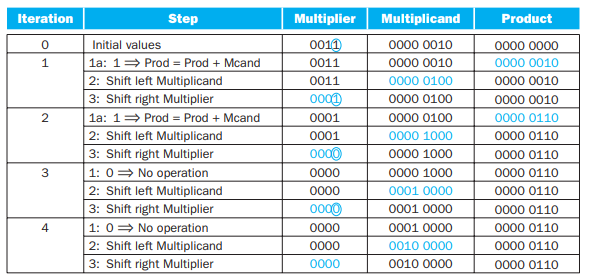
\includegraphics[scale = 0.8]{q6_table.png}
            \caption{Multiply example}
        \end{center}
    \end{figure}
    \begin{solution}
        (40)$_8$ = (100000)$_2$, (60)$_8$ = (000000110000)$_2$. (40)$_8$ x (60)$_8$ = (3000)$_8$. 
        \begin{tabular}{|c|c|c|c|c|}
            \hline
            \rowcolor{cyan}
            \textcolor{white}{Iteration}& \textcolor{white}{Step} & \textcolor{white}{Multiplier} & \textcolor{white}{Multiplicand} & \textcolor{white}{Product} \\ \hline
            0 & Initial values & 10000\textcircled{0} &  000000 110000 & 000000 000000 \\ \hline 
            \multirow{5}{*}{1} & 0 $\rightarrow$ No operation & 100000 & 000000 110000 & \textcolor{cyan}{000000 000000} \\ 
            & Shift left Multiplicand & 100000 & \textcolor{cyan}{000001 100000} & 000000 000000 \\ 
            & Shift right Multiplier & \textcolor{cyan}{01000\textcircled{0}} & 000001 100000 & 000000 000000 \\ \hline
            \multirow{5}{*}{2} & 0 $\rightarrow$ No operation & 010000 & 000001 100000 & \textcolor{cyan}{000000 000000} \\
            & Shift left Multiplicand & 010000 & \textcolor{cyan}{000011 000000} & 000000 000000 \\ 
            & Shift right Mulitplier & \textcolor{cyan}{00100\textcircled{0}} & 000011 000000 & 000000 000000 \\ \hline
            \multirow{5}{*}{3} & 0 $\rightarrow$ No operation & 001000 & 000011 000000 & \textcolor{cyan}{000000 000000} \\
            & Shift left Multiplicand & 001000 & \textcolor{cyan}{000110 000000} & 000000 000000 \\ 
            & Shift right Multiplier & \textcolor{cyan}{00010\textcircled{0}} & 000110 000000 & 000000 000000 \\ \hline
            \multirow{5}{*}{4} & 0 $ \rightarrow$ No operation & 000100 & 000110 000000 & \textcolor{cyan}{000000 000000} \\ 
            & Shift left Multiplicand & 000100 & \textcolor{cyan}{001100 000000} & 000000 000000 \\ 
            & Shift right Multipler & \textcolor{cyan}{00001\textcircled{0}} & 001100 000000 & 000000 000000 \\ \hline
            \multirow{5}{*}{5} & 0 $\rightarrow$ No operation & 000010 & 001100 000000 & 000000 000000 \\ 
            & Shift left Multiplicand & 000010 & \textcolor{cyan}{011000 000000} & 000000 000000 \\ 
            & Shift right  Multiplier & \textcolor{cyan}{00000\textcircled{1}} & 011000 000000 & 000000 000000 \\ \hline
            \multirow{5}{*}{6} & 1 $\rightarrow$ Prod = Prod + Mcand & 000001 & 011000 000000 & \textcolor{cyan}{011000 000000} \\ 
            & Shift left Multiplicand & 000001 & \textcolor{cyan}{110000 000000} & 011000 000000 \\ 
            & Shift right Multiplier & \textcolor{cyan}{000000} & 110000 000000 & 011000 000000 \\ \hline
        \end{tabular}
        
        Result (011000 000000)$_2$ = (3000)$_8$ which is the required output.
    \end{solution}
\pagebreak
    \question[15]\textbf{Q7} [15 marks] \\ 
    Given the RISC-V processor implementation below, answer the following: 
    \begin{figure}[h]
        \begin{center}
            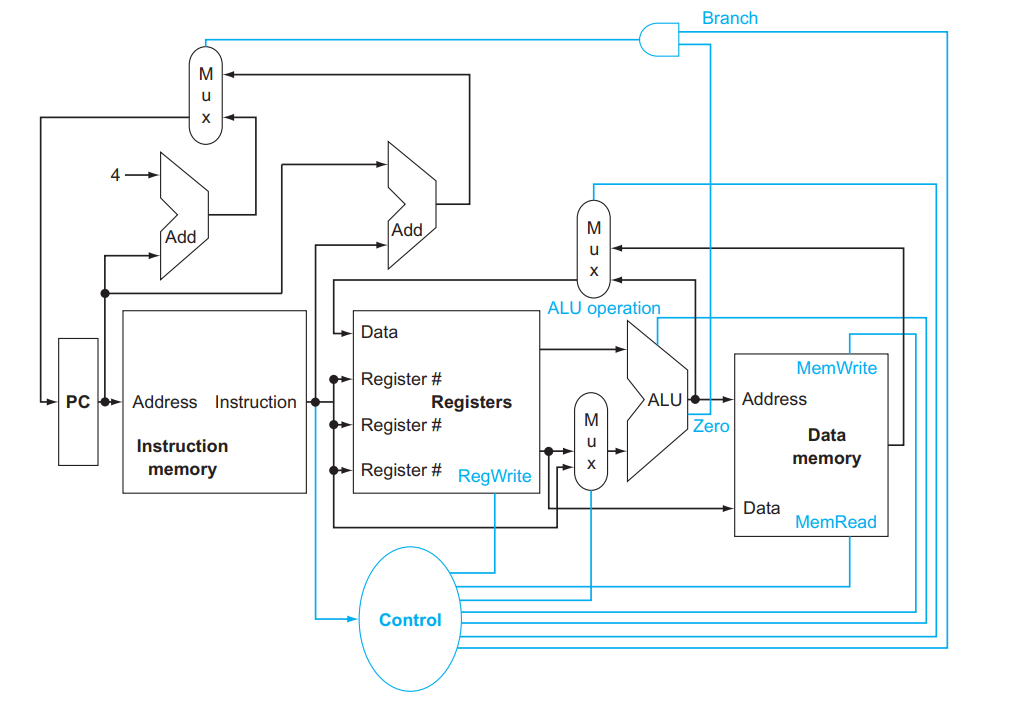
\includegraphics[scale = 0.5]{q7_fig.png}
            \caption{Basic implementation of the RISC-V subset, including the necessary multiplexors and control lines.}
        \end{center}
    \end{figure}
    \begin{parts}
        \part Explain what is meant by a single cycle data path. 
        \part Explain the working of the Control Unit, and why it is needed?
        \part Explain in as much detail as possible, the process of accessing the next instruction, which elements of the above processor are used, and why?
        \part Explain the purpose of each of the multiplixers, as they are labeled, in the given processor.
    \end{parts}
    \begin{solution}
        \begin{parts}
            \part A datapath is the part of the processor that contains the hardware necessary to perform the required operations. \\ A single cycle datapath executes in one single clock cycle all the instructions that the datapath is designed to implement. So one complete instruction is executed in one clock ``tick''. This means that the processor can fetch an instruction from the memory, decode it, execute it, and write the result back [if needed] all in one single clock cycle. 
            % The significance of this is that each single clock ``tick'' would take the same time, and each instruction is executed in a single clock cycle, therefore, each instruction would take the same amount of time to execute. Hence, the CPI remains same for all instructions. 
            \part The Control Unit is one of the most important components of the architecture, responsible for controlling the flow of data and instructions within the processor. Its primary function is to generate control signals that coordinate the operation of all the other components within the CPU, including the ALU, memory, and registers. It has an instruction as an input, and is used to determine how to set the control lines for the functional units and the multiplexors. The Control Unit will also ensure the tasks are executed in the correct order. According to the instruction it decodes, it will send a signal to \texttt{RegWrite} in case a data is to be written in a register, sends a signal for branch conditions, ALUop for ALU operations to name a few. \\ In short, it is needed to ensure that the CPU functions correctly and performs the operations required by the instruction.

            \part The PC [Program Counter] holds the adress of the next instruction to be fetched. The instruction memory contains the program instructions. The PC first sends the address of the instruction, and then the instruction is fetched from the Instruction Memory and sent to the Register File, and Control Unit. The Control Unit decodes the instruction and determines accordingly which signals are to be activated; RegWrite in case data is to be written on a register, ALUSrc to determine which values to be sent to the ALU from ReadData 2 or immediate, ALUop to determine the operation to be performed by the ALU, MemRead to determine whether data is to be read from memory, MemWrite to determine if data is to be written onto Memory, and Branch in case there is a branch condition. Accordingly, different components will be accessed or not accessed, but Register File, ALU, and Instruction Memory will always be used. Once the required operations are done, a signal is sent to the top most MUX, which depending upon the Branch condition will either send the address of the next instruction to the PC by taking in the incremented value of the address and the next instruction is accessed, or sends the value of the branch instruction address in which case the branch address is passed and the next instruction - branch instruction - is fetched from the Instruction Memory. 

            \part \textbf{The top multiplexor} determines what value is replaced into the Program Counter (PC); PC + 4 in case we need to move onto the next instruction, or branch destination address in case there was a branch in the instruction. 
            % Branch is determined by ``ANDing'' the Zero output from the ALU[\texttt{beq} instruction], and control signal generated by the Control Unit which indicates it is a branch. 
            
            \textbf{The middle multiplexor} takes input from the ALU, and the Data Memory, along with a select line from the Control Unit, and based on the signal from the Control Unit, it decides which type of data is to be written in the register file; output of the ALU in case of arithmetic logic instructions, or output of the Data Memory in case of load for writing into the register file. 

            \textbf{The bottom multiplexor} is used to determine the input that is taken by the ALU; the input can be from the register file in case of arithmetic-logical instruction or branch instruction, or from the offset of the instruction in case of load/store instruction (again a signal is sent from the Control Unit that acts as the select line for this multiplexor).
        \end{parts}
    \end{solution}
\pagebreak
    \question[15]\textbf{Q8} [15 marks] \\ 
    Given the RISC-V processor implementation below, answer the following:
    \begin{figure}[h]
        \begin{center}
            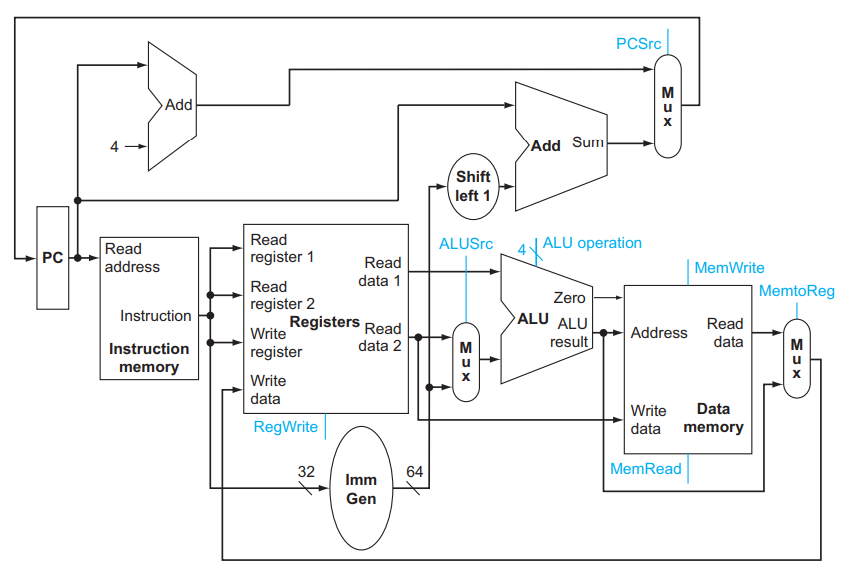
\includegraphics[scale = 0.5]{q8_fig.png}
            \caption{The simple datapath for the core RISC-V architecture combines the elements
            required by different instruction classes}
        \end{center}
    \end{figure}
    \begin{parts}
        \part For the instructions below, identify the components of the processor it uses and what are the values of MemRead, MemWrite, RegWrite, and MemtoReg.
        \begin{subparts}
            \subpart add x5, x6, x7
            \subpart ld x5, 64(x2)
            \subpart sd x6, 80(x2)
            \subpart addi x5, x6, 5
        \end{subparts}
        \part To support branch instructions, what must be added to the processor shown above? What other components of the processor are used when a branch instruction is being run and why are they used?
        \part In reference to the above processor implementation, explain the significance and benefit of the generalization of the RISC V instruction format.
    \end{parts}
    \begin{solution}
        \begin{parts}
            \part \begin{subparts}
                \subpart add x5, x6, x7 \begin{enumerate}
                    \item Instruction Memory to fetch instruction 
                    \item PC to get address of the instruction 
                    \item Register File to read Register values from Register 1 and Register 2, and write data onto destination register 
                    \item ALU to perform necessary arithmetic 
                \end{enumerate} 
                
                % It uses the Instruction Memory - fetch instruction, PC[Program Counter] - increment for the next instruction, Register File - takes Read Register 1, Read Register 2, Write Register and Write data, and sends Read data 1 and Read Data 2 to ALUSrc MUX and ALU. ALU - performs necessary arithmetic and sends the result to MUX which is then forwarded to Write Data on destination register in the Register File.
                MemRead, MemWrite and MemtoReg are 0. RegWrite = 1. 
                % MemRead is 0, since we are not loading anything from memory. MemWrite is 0 since we are not storing or writing anything onto memory. RegWrite is 1 since the data is written onto the destination register. MemtoReg is 0 since the output is not to be written back onto the register.
                \subpart ld x5, 64(x2) \begin{enumerate}
                    \item Instruction Memory to fetch instruction 
                    \item PC to get address of the instruction 
                    \item Register File to read Register value from Register 1 and write data onto destination register
                    \item Imm Gen to extract immediate value for the offset 
                    \item ALU to perform necessary arithmetic
                    \item Data Memory to forward the daat from the address onto Register File 
                \end{enumerate} 
                MemRead, RegWrite and MemtoReg = 1. MemWrite = 0.
                % It uses the Instruction Memory - fetch instructions, PC[Program Counter] - increment for the next instruction, Register File - takes Read Register 1, Write Register and Write Data, and sends Read Data 1 to the ALU. The Imm Gen takes the instruction as well and sends the immediate value to the ALU for the offset on the base address in the register. The MUX takes in the value of Imm Gen and forwards it to the ALU. The ALU takes Read Data 1 from Register File and Imm Gen value and adds the offset to the address, and sends the result to the Data Memory. The Data Memory takes the address and forwards the data from the address as Read Data to the MUX which in turn passes data to the Write Data where the data is written onto the destination register[Write Register] in the Register File. 
                % MemRead is 1 since we have to read data in the address from the memory. MemWrite is 0 as we are not writing anything to memory. RegWrite is 1 as data is written onto the destination register. MemtoReg is 1 since the output is written back onto the register.
                \subpart sd x6, 80(x2) \\ The sd [store doubleword] works almost the same way as the ld [load doublword] works. However, sd would indicate a write operation rather than a read operation, the second register value would be used for data to store, and the operation of writing the data memory value to register file would not occur. \\ MemRead and RegWrite = 0. MemWrite = 1. MemtoReg = x [don't care] 
                % So, MemRead would be 0, MemWrite would be 1 as we are writing the data to memory. RegWrite would be 0 as we are not writing data onto a register. MemtoReg would be ``x'' meaning it would be don't care since the register is not being written, the value of the data on the register data write port is not used.
                \subpart addi x5, x6, 5 \\ The addi [add immediate] works very similar to the add instruction. The main difference is that Imm Gen would take the instruction and send the immediate value to the MUX which in turn sends the immediate value to the ALU to perform the addition with the ReadData 1 value it takes from the Register File. The ALU result would be sent to the MUX and the MUX sends the data to the Write Data of Register File to write data on the destination register. \\ 
                MemRead, MemWrite, and MemtoReg = 0. RegWrite = 1. 
                % MemRead would be 0 since data is not read from memory. MemWrite is also 0 as data is not written onto memory. RegWrite is 1 as data is being written onto the destination register. MemtoReg is also 0.   
            \end{subparts}
            \part A branch instruction: beq x1, x2, offset 
            
            The instruction is fetched from the Instruction memory and the PC is incremented. The instruction is sent to the Register File which takes two values of Read Register 1 and Read Register 2. There is no destination register, so Write Register is not used. There is, however, the offset [an immediate] which is generated from the Imm Gen. The Register File also sends output as Read Register 1 and Read Register 2 to the ALU which compares the two values to determine the branch condition. Since data is not being read or written from the memory, so Data Memory is not used. The ALU result of ``Zero'' must be sent to an ``AND'' gate, that also takes in a ``branch'' value. A branch signal would be sent if there is a branch, and in case the ALU sends a branch condition, then the ``AND'' gate sends an output signal to a MUX which in turn sends an output to the PC. The ``Zero'' value decides which adder result to store in the PC. Depending upon the ``Zero'' the ``AND'' would either give a 0 or a 1 which would decide whether the branch is not equal, in which case the PC is incremented to the next instruction, or if the branch is equal, in which case the PC is given the value of the address of the branch condition. 

            MemRead and MemWrite would be 0, RegWrite would be 0, an additional signal of ``branch'' would be 1, MemtoReg would be x [don't care].

            \part The significance and benefit of this generalization is that it provides consistency to the system, and does not require any additional components to perform differnet/specific tasks which reduces complexity as it can support a wide range of instructions with a single instruction format. Moreover, it can also support a wide range of applications, as the instruction format is generalized so is able to accomodate various operations, operand types, addressing modes, and encoding formats - not limited to R-Type or any other specific format. This also makes the design much more flexible and enables the development of custom instructions designed to handle specific tasks. The aforementioned results in efficient encoding of instructions as the instruction format can be designed to minimize or extend the number of bits required to encode an instruction.  
        \end{parts}
    \end{solution}
    % \pagebreak
    \question[10]\textbf{Q9} [10 marks] \\ 
    On a Single Cycle Processor, \\ Consider the following instruction mix:
    
    \begin{tabular}{|c|c|c|c|c|c|}
        \hline
        \hspace*{3.20mm}\textbf{R-type}\hspace*{3.20mm} & \hspace*{3.20mm}\textbf{I-type(non-LD)}\hspace*{3.20mm} & \hspace*{3.20mm}\textbf{Load}\hspace*{3.20mm} & \hspace*{3.20mm}\textbf{Store}\hspace*{3.20mm} & \hspace*{3.20mm}\textbf{Branch}\hspace*{3.20mm} & \hspace*{3.20mm}\textbf{Jump}\hspace*{3.20mm} \\ \hline
        20\% & 16\% & 30\% & 18\% & 9\% & 7\% \\ \hline
    \end{tabular}
    \begin{parts}
        \part What fraction of all instructions use data memory?
        \part What fraction of all instructions use instruction memory?
        \part What fraction of all instructions use the sign extend?
        \part What is the sign extend doing during cycles in which its output is not needed.
    \end{parts}

    \begin{solution}
        \begin{parts}
            \part Data Memory is used by Load and Store instructions. Therefore, Data Memory is used by $30 + 18 = 48\%$ of all instruction. 
            \part Instruction Memory contains the instructions, therefore, every instruction has to be fetched from the instruction memory. So $100\%$ of instructions use instruction memory.
            \part R-Type instructions only operate on the register values which are already of fixed size and do not require sign extension. Sign extension is used by I-Type and S-Type instructions that involve Load, Store, Branch or Jump instructions. So apart from R-Type, the remaining instructions use sign extend. So $100 - 20 = 80\%$ of instructions use sign extend. 
            \part Sign extend value is computed on each cycle and is sent to the MUX. If its value is needed, it is passed on else its value is not picked up and ignored.
        \end{parts}
    \end{solution}

\end{questions}
\end{sloppypar}
\end{document}